\documentclass[12pt]{article}
\usepackage[utf8]{inputenc}
\usepackage{amsmath}
\usepackage{amssymb}
\usepackage{geometry}
\usepackage{listings}
\usepackage{xcolor}
\usepackage{hyperref}
\usepackage{booktabs}
\usepackage{array}
\usepackage{graphicx}
\usepackage{float}
\usepackage{enumitem}
\usepackage{tikz}
\usetikzlibrary{matrix,positioning,arrows.meta}

\geometry{a4paper, margin=1in}

\definecolor{codegreen}{rgb}{0,0.6,0}
\definecolor{codegray}{rgb}{0.5,0.5,0.5}
\definecolor{codepurple}{rgb}{0.58,0,0.82}
\definecolor{backcolour}{rgb}{0.95,0.95,0.92}

\lstset{
    backgroundcolor=\color{backcolour},
    commentstyle=\color{codegreen},
    keywordstyle=\color{magenta},
    numberstyle=\tiny\color{codegray},
    stringstyle=\color{codepurple},
    basicstyle=\ttfamily\small,
    breakatwhitespace=false,
    breaklines=true,
    captionpos=b,
    keepspaces=true,
    numbers=left,
    numbersep=5pt,
    showspaces=false,
    showstringspaces=false,
    showtabs=false,
    tabsize=2,
    language=Python
}

\title{%
    \large 8th Semester Artificial Intelligence Laboratory 2026 \\[4pt]
    \large CS 4271 \\[10pt]
    \textbf{\LARGE ASSIGNMENT -- 6} \\[8pt]
    \textbf{\Large AGV Navigation in a Smart Fulfillment Center} \\[4pt]
    \large Tabular Q-Learning with $\varepsilon$-Greedy Exploration
}
\author{Uttam Mahata (2022CSB104)}
\date{\today}

\begin{document}

\maketitle
\tableofcontents
\newpage

% -----------------------------------------------------------------------------
\section{Introduction}
% -----------------------------------------------------------------------------

An Autonomous Guided Vehicle (AGV) must navigate a \textbf{6$\times$6 warehouse
grid} from a charging station to a shipping dock while avoiding hazardous zones.
The AGV begins with no knowledge of the floor plan and must discover safe paths
entirely through experience.

This assignment implements a \textbf{tabular Q-learning} agent --- a
model-free reinforcement learning algorithm --- to solve this navigation
problem. Through repeated interaction with the environment the agent learns an
action-value function that enables it to choose optimal, collision-free routes.

Key features of this implementation:
\begin{itemize}
    \item Deterministic $6 \times 6$ grid-world with 36 discrete states.
    \item Four-action movement (Up, Down, Left, Right) with solid boundary walls.
    \item Three hazard cells yielding severe penalties: $(2,2)$, $(2,3)$, $(3,2)$.
    \item $\varepsilon$-greedy exploration with exponential decay from
          $\varepsilon = 1.0$ to $\varepsilon = 0.01$ over 1000 episodes.
    \item Three output visualisations: Q-tables, learning curves, and optimal
          path overlay.
\end{itemize}

% -----------------------------------------------------------------------------
\section{Problem Formulation}
% -----------------------------------------------------------------------------

\subsection{Grid Environment}

The warehouse floor is abstracted as a discrete 2-D grid of size $6 \times 6$.
Each cell is addressed by a coordinate pair $(x, y)$ where $x$ is the column
and $y$ is the row. The origin $(0,0)$ is the \emph{top-left} corner and
$(5,5)$ is the \emph{bottom-right} corner.

\begin{center}
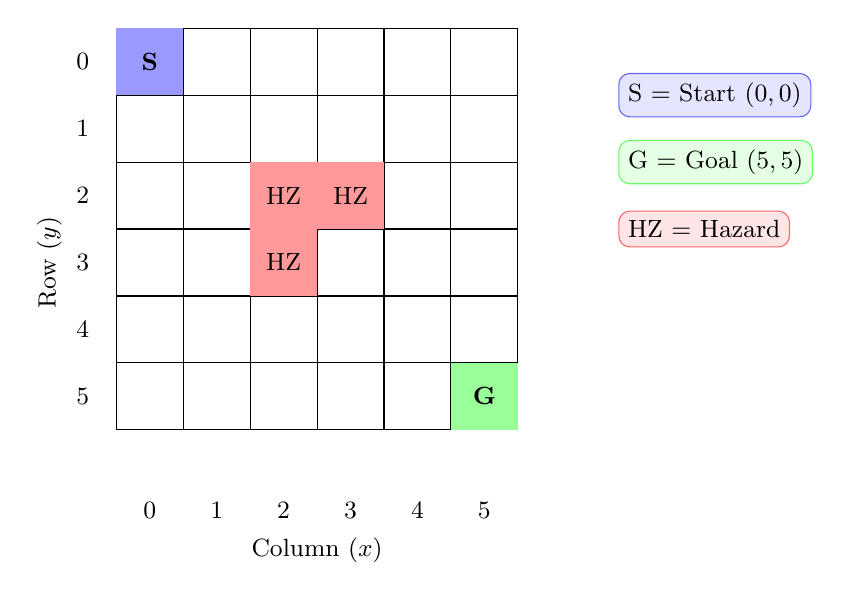
\begin{tikzpicture}[scale=0.85]
    \foreach \x in {0,...,5} {
        \foreach \y in {0,...,5} {
            \draw (\x, -\y) rectangle (\x+1, -\y+1);
        }
    }
    \fill[blue!40]  (0,0) rectangle (1,1);
    \fill[green!40] (5,-5) rectangle (6,-4);
    \fill[red!40]   (2,-2) rectangle (3,-1);
    \fill[red!40]   (2,-3) rectangle (3,-2);
    \fill[red!40]   (3,-2) rectangle (4,-1);

    \node at (0.5, 0.5)  {\small\textbf{S}};
    \node at (5.5,-4.5)  {\small\textbf{G}};
    \node at (2.5,-1.5)  {\small HZ};
    \node at (2.5,-2.5)  {\small HZ};
    \node at (3.5,-1.5)  {\small HZ};

    \foreach \x in {0,...,5} {
        \node at (\x+0.5, -6.2) {\small\x};
    }
    \foreach \y in {0,...,5} {
        \node at (-0.5, -\y+0.5) {\small\y};
    }
    \node at (3, -6.8) {\small Column ($x$)};
    \node[rotate=90] at (-1.0, -2.5) {\small Row ($y$)};

    \node[draw=blue!60, fill=blue!10,  rounded corners, right] at (7.5, 0)   {\small S~=~Start $(0,0)$};
    \node[draw=green!60,fill=green!10, rounded corners, right] at (7.5,-1.0) {\small G~=~Goal $(5,5)$};
    \node[draw=red!60,  fill=red!10,   rounded corners, right] at (7.5,-2.0) {\small HZ = Hazard};
\end{tikzpicture}
\end{center}

\subsection{State Space}

The state space $\mathcal{S}$ consists of the 36 grid cells:
\[
    \mathcal{S} = \{(x, y) \mid x,y \in \{0,1,2,3,4,5\}\}
\]
Each state is mapped to a flat index $s = y \cdot 6 + x \in \{0, \ldots, 35\}$
for storage in the Q-table.

\subsection{Action Space}

At every state the AGV may take one of four deterministic actions:
\[
    \mathcal{A} = \{\textit{Up},\;\textit{Down},\;\textit{Left},\;\textit{Right}\}
\]

Action deltas in $(dx, dy)$ form (with $y$ increasing downward):

\begin{center}
\begin{tabular}{@{} l c c @{}}
\toprule
\textbf{Action} & $dx$ & $dy$ \\
\midrule
Up    &  0 & $-1$ \\
Down  &  0 & $+1$ \\
Left  & $-1$ & 0 \\
Right & $+1$ & 0 \\
\bottomrule
\end{tabular}
\end{center}

Attempting to move off the grid boundary leaves the AGV in its current state.

\subsection{Terminal State}

The episode terminates when the AGV reaches the goal cell $(5,5)$.
Entering a hazard cell does \emph{not} terminate the episode --- it applies a
penalty and the AGV continues from the hazard cell.

% -----------------------------------------------------------------------------
\section{Reward Structure}
% -----------------------------------------------------------------------------

The reward function provides immediate feedback after each action:

\begin{table}[H]
\centering
\begin{tabular}{@{} l c l @{}}
\toprule
\textbf{Event} & \textbf{Reward} & \textbf{Termination} \\
\midrule
Reach goal $(5,5)$         & $+100$ & Yes \\
Enter hazard cell          & $-50$  & No  \\
Any other (safe) step      & $-1$   & No  \\
Hit a boundary wall        & $-1$   & No  \\
\bottomrule
\end{tabular}
\caption{Immediate reward function $R(s, a, s')$.}
\end{table}

The $-1$ step penalty is critical: it penalises every wasted movement and
forces the agent to discover the \emph{shortest} safe path rather than
wandering indefinitely.

% -----------------------------------------------------------------------------
\section{Q-Learning Algorithm}
% -----------------------------------------------------------------------------

\subsection{Overview}

Q-learning is an \emph{off-policy}, \emph{model-free}
temporal difference (TD) method. It directly estimates the optimal
action-value function $Q^*(s, a)$ without requiring a model of transition
probabilities.

\subsection{Q-Table Initialisation}

A table $Q \in \mathbb{R}^{36 \times 4}$ is maintained, mapping every
(state, action) pair to an estimated cumulative return. All entries are
initialised to zero:
\[
    Q(s, a) = 0 \quad \forall\; s \in \mathcal{S},\; a \in \mathcal{A}
\]

\subsection{Bellman Update Rule}

After executing action $A_t$ in state $S_t$, observing reward $R_{t+1}$ and
transitioning to state $S_{t+1}$, the Q-value is updated via:

\begin{equation}\label{eq:bellman}
    Q(S_t, A_t) \;\leftarrow\; Q(S_t, A_t)
    + \alpha \Bigl[
        R_{t+1} + \gamma \max_{a'} Q(S_{t+1}, a') - Q(S_t, A_t)
    \Bigr]
\end{equation}

where:
\begin{itemize}
    \item $\alpha = 0.1$ is the \textbf{learning rate} --- controls how much
          new information overwrites old estimates.
    \item $\gamma = 0.9$ is the \textbf{discount factor} --- weights future
          rewards relative to immediate ones.
    \item $\max_{a'} Q(S_{t+1}, a')$ is the \textbf{greedy bootstrap} --- the
          best estimated value reachable from the next state.
    \item $R_{t+1} + \gamma \max_{a'} Q(S_{t+1}, a') - Q(S_t, A_t)$ is the
          \textbf{TD error}.
\end{itemize}

When the episode terminates (goal reached), no future value exists, so the
update simplifies to:
\[
    Q(S_t, A_t) \leftarrow Q(S_t, A_t) + \alpha\bigl[R_{t+1} - Q(S_t, A_t)\bigr]
\]

\subsection{$\varepsilon$-Greedy Exploration}

The agent uses an \textbf{$\varepsilon$-greedy} strategy to balance exploration
and exploitation:

\[
    A_t =
    \begin{cases}
        \text{random action from } \mathcal{A} & \text{with probability } \varepsilon \\
        \arg\max_{a} Q(S_t, a)                  & \text{with probability } 1 - \varepsilon
    \end{cases}
\]

$\varepsilon$ decays exponentially after each episode:
\[
    \varepsilon_k = \max\!\bigl(\varepsilon_{\min},\;
                                \varepsilon_0 \cdot \delta^k\bigr)
\]

with $\varepsilon_0 = 1.0$, $\varepsilon_{\min} = 0.01$, and decay factor
$\delta = 0.995$. This guarantees full exploration early in training and
near-complete exploitation by episode~900.

\begin{table}[H]
\centering
\begin{tabular}{@{} l c @{}}
\toprule
\textbf{Episode} & \textbf{$\varepsilon$ value} \\
\midrule
0   & 1.000 \\
100 & 0.607 \\
300 & 0.223 \\
500 & 0.082 \\
700 & 0.030 \\
900 & 0.011 $\approx \varepsilon_{\min}$ \\
\bottomrule
\end{tabular}
\caption{Epsilon schedule over 1000 training episodes.}
\end{table}

\subsection{Algorithm Pseudocode}

\begin{lstlisting}[language={}, caption={Tabular Q-Learning (pseudocode)}, mathescape=true]
Initialise: Q(s,a) = 0 for all s,a
            $\varepsilon$ = 1.0

for episode k = 1 to 1000:
    $\varepsilon_k$ = max($\varepsilon_{min}$, $\varepsilon_0 \cdot \delta^k$)
    s = START

    for step t = 1 to MAX_STEPS:
        with prob $\varepsilon_k$: a = random action    // explore
        else:          a = argmax_a' Q(s, a')  // exploit

        s', r, done = env.step(s, a)

        if done:
            Q(s,a) += $\alpha$ * (r - Q(s,a))
        else:
            Q(s,a) += $\alpha$ * (r + $\gamma$ * max_a'' Q(s',a'') - Q(s,a))

        s = s'
        if done: break
\end{lstlisting}

% -----------------------------------------------------------------------------
\section{Implementation}
% -----------------------------------------------------------------------------

\subsection{Module Structure}

\begin{lstlisting}[caption={Layout of agv\_navigation.py}]
agv_navigation.py
|- Constants          (GRID_SIZE, START, GOAL, HAZARDS, ACTIONS,
|                      ALPHA, GAMMA, EPS_START, EPS_MIN, EPS_DECAY,
|                      EPISODES, MAX_STEPS)
|- WarehouseEnv                   # grid environment
|   |- state_to_idx(x, y)        # (x,y) -> flat index 0-35
|   |- idx_to_state(idx)         # flat index -> (x,y)
|   |- reset()                   # return START index
|   |- step(state_idx, action)   # (next_idx, reward, done)
|- QLearningAgent                 # Q-learning agent
|   |- q_table                   # numpy (36,4) array
|   |- choose_action(s, epsilon) # epsilon-greedy selection
|   |- greedy_action(s)          # argmax Q[s]
|   |- update(s, a, r, s', done) # Bellman update
|- train(agent, env, episodes)   # training loop
|- print_q_table(...)            # formatted Q-table display
|- print_best_actions_grid(...)  # ASCII policy grid
|- get_optimal_path(...)         # greedy path extraction
|- print_path_ascii(...)         # ASCII path overlay
|- plot_reward_curve(...)        # matplotlib Plot 2
|- plot_optimal_action_curve(...)# matplotlib Plot 1
|- plot_optimal_path(...)        # matplotlib grid + arrows
|- main()                        # entry point
\end{lstlisting}

\subsection{State Indexing}

States are stored using row-major (C-order) flattening:
\[
    \text{idx}(x, y) = y \times 6 + x, \qquad
    (x, y) = \bigl(\text{idx} \bmod 6,\;\lfloor\text{idx}/6\rfloor\bigr)
\]

\begin{lstlisting}[caption={State encoding in WarehouseEnv.}]
@staticmethod
def state_to_idx(x: int, y: int) -> int:
    return y * GRID_SIZE + x

@staticmethod
def idx_to_state(idx: int):
    return (idx % GRID_SIZE, idx // GRID_SIZE)
\end{lstlisting}

\subsection{Environment Step}

\begin{lstlisting}[caption={Transition and reward logic in WarehouseEnv.step.}]
def step(self, state_idx: int, action: int):
    x, y = self.idx_to_state(state_idx)
    dx, dy = ACTION_DELTA[action]

    nx = max(0, min(GRID_SIZE - 1, x + dx))
    ny = max(0, min(GRID_SIZE - 1, y + dy))
    next_state = (nx, ny)
    next_state_idx = self.state_to_idx(nx, ny)

    if next_state == GOAL:
        return next_state_idx, REWARD_GOAL, True
    elif next_state in HAZARDS:
        return next_state_idx, REWARD_HAZARD, False
    else:
        return next_state_idx, REWARD_STEP, False
\end{lstlisting}

\subsection{Bellman Update}

\begin{lstlisting}[caption={Q-value update in QLearningAgent.update.}]
def update(self, s: int, a: int, r: float, s_next: int, done: bool):
    future_value = 0.0 if done else GAMMA * np.max(self.q_table[s_next])
    td_error = r + future_value - self.q_table[s, a]
    self.q_table[s, a] += ALPHA * td_error
\end{lstlisting}

\subsection{Training Loop (core)}

\begin{lstlisting}[caption={Per-episode training logic inside train().}]
for ep in range(episodes):
    epsilon = max(EPS_MIN, EPS_START * (EPS_DECAY ** ep))
    state   = env.reset()

    for _ in range(MAX_STEPS):
        is_greedy = (random.random() >= epsilon)
        if is_greedy:
            action = agent.greedy_action(state)
        else:
            action = random.randint(0, NUM_ACTIONS - 1)

        next_state, reward, done = env.step(state, action)
        agent.update(state, action, reward, next_state, done)
        state = next_state
        if done:
            break
\end{lstlisting}

% -----------------------------------------------------------------------------
\section{Results}
% -----------------------------------------------------------------------------

\subsection{Initial Q-Table}

Before training begins all 36$\times$4 = 144 entries are zero.
The agent has no preference among actions and explores purely at random
($\varepsilon = 1.0$).

\subsection{Convergence}

After 1000 training episodes the following statistics are observed:

\begin{center}
\begin{tabular}{@{} l r @{}}
\toprule
\textbf{Metric} & \textbf{Value} \\
\midrule
Final $\varepsilon$             & 0.0100 \\
Last-100 average episode reward & $\approx +90$ \\
Last-100 \% greedy actions      & $\approx 99\%$ \\
Optimal path length             & 10 steps \\
\bottomrule
\end{tabular}
\end{center}

Notable learned Q-values:
\begin{itemize}
    \item $Q\bigl((5,4),\,\textit{Down}\bigr) = +100$ --- the cell immediately
          above the goal correctly learns that moving Down yields a terminal
          reward of $+100$ with no discounting (one-step to goal).
    \item $Q\bigl((5,5),\,\cdot\bigr) = 0$ --- the terminal state has no
          future value, so all entries remain zero as expected.
    \item Hazard-adjacent cells accumulate strong negative Q-values for
          actions pointing into hazard cells, effectively building an
          implicit obstacle map.
\end{itemize}

\subsection{Learning Curve: Average Reward vs.\ Episodes}

\begin{figure}[H]
\centering
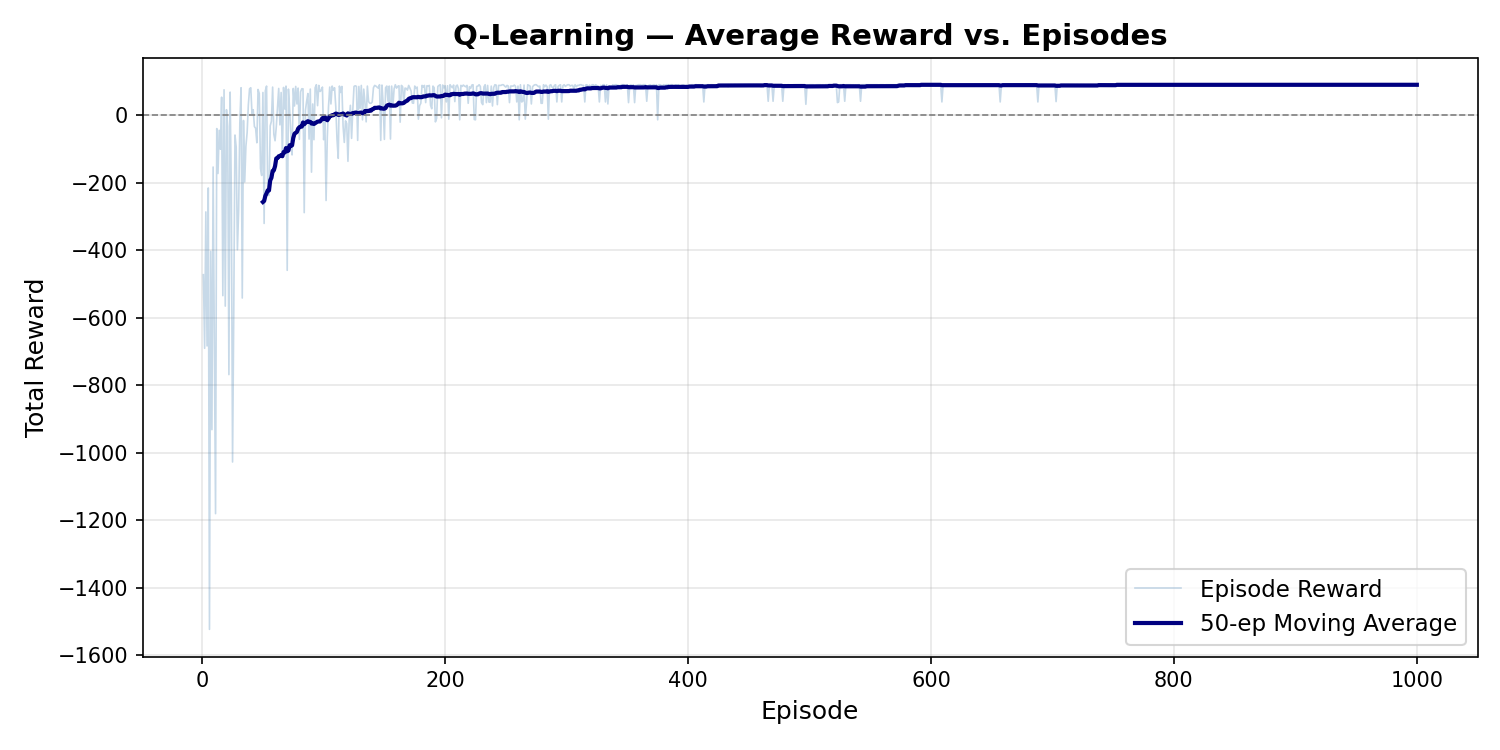
\includegraphics[width=0.92\textwidth]{q_learning_rewards.png}
\caption{Total reward per episode (light blue) and 50-episode moving average
         (navy). The reward rises from near $-200$ in early random episodes
         to $\approx +90$ as the agent learns the optimal path.}
\end{figure}

\subsection{Learning Curve: \% Optimal Actions vs.\ Episodes}

\begin{figure}[H]
\centering
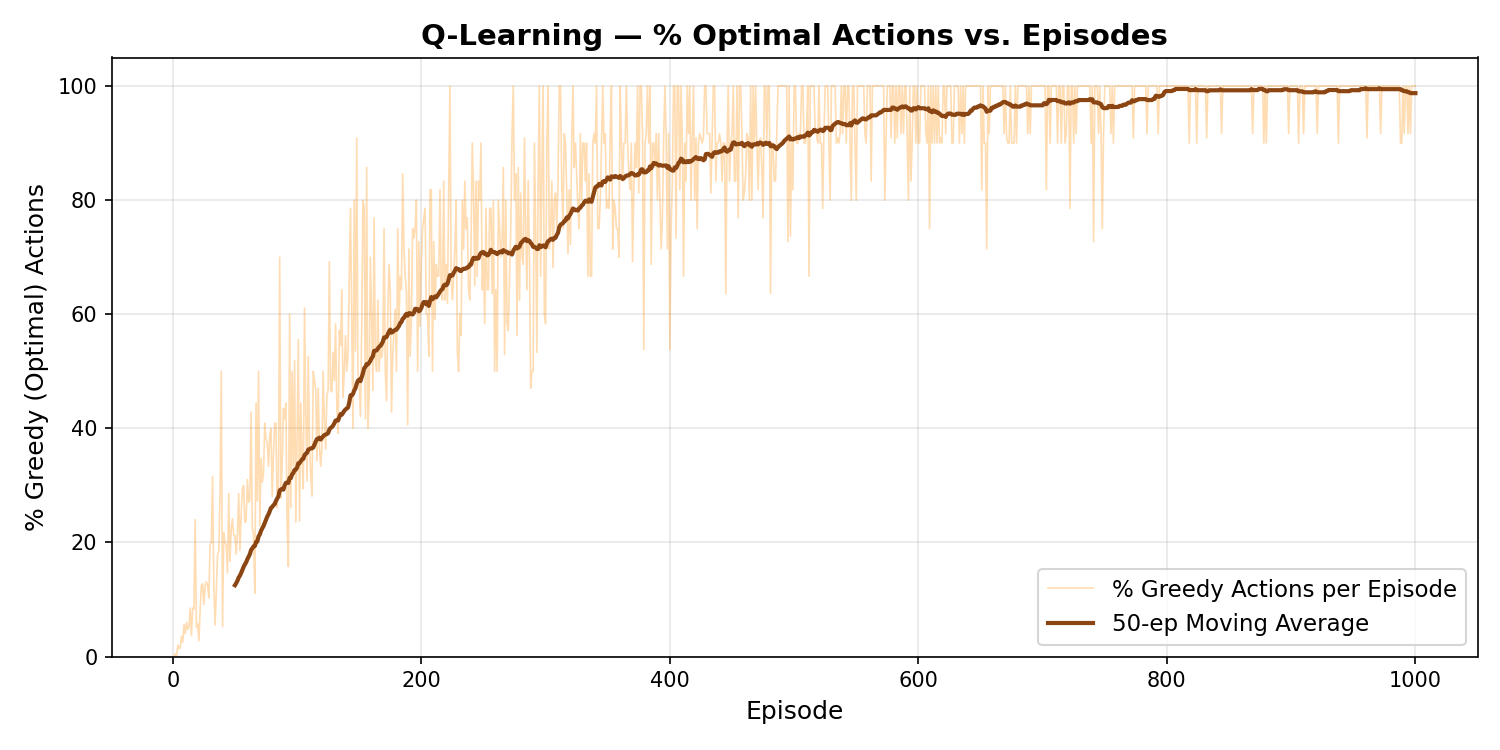
\includegraphics[width=0.92\textwidth]{q_learning_optimal_actions.png}
\caption{Percentage of steps where the agent chose the greedy (highest Q-value)
         action. Rises monotonically as $\varepsilon$ decays, reaching $\sim$99\%
         by episode 900.}
\end{figure}

\subsection{Optimal Path}

\begin{figure}[H]
\centering
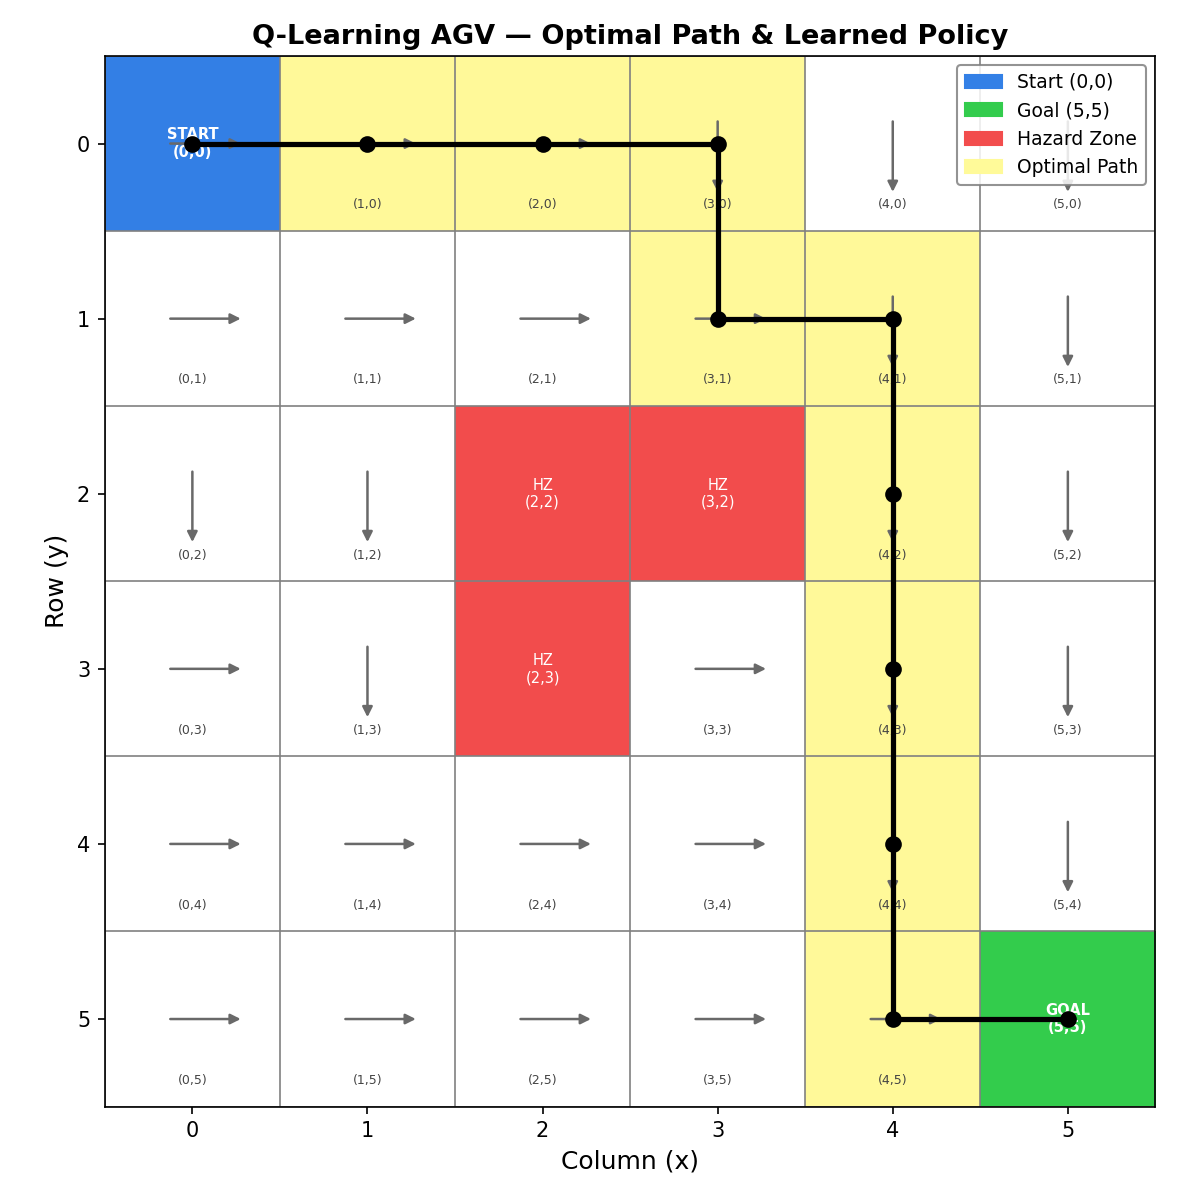
\includegraphics[width=0.78\textwidth]{optimal_path.png}
\caption{Learned policy arrows overlaid on the 6$\times$6 grid. The bold black
         line traces the 10-step optimal path. Red cells are hazard zones, blue
         is the start, green is the goal, and yellow cells lie on the path.}
\end{figure}

The fully trained agent follows a 10-step collision-free path:
\[
(0,0) \to (1,0) \to (2,0) \to (3,0) \to (3,1) \to (4,1)
      \to (4,2) \to (4,3) \to (4,4) \to (4,5) \to (5,5)
\]

The path hugs the right side of the hazard cluster, navigating around all
three forbidden cells $(2,2)$, $(2,3)$, and $(3,2)$.

% -----------------------------------------------------------------------------
\section{Complexity Analysis}
% -----------------------------------------------------------------------------

\begin{table}[H]
\centering
\begin{tabular}{@{} l l l @{}}
\toprule
\textbf{Component} & \textbf{Time} & \textbf{Space} \\
\midrule
Q-table storage              & $O(|\mathcal{S}| \cdot |\mathcal{A}|)$ & 36$\times$4 = 144 floats \\
Per-step update              & $O(|\mathcal{A}|)$ for $\max_{a'}$      & $O(1)$ \\
Per-episode (max steps)      & $O(T_{\max} \cdot |\mathcal{A}|)$       & $O(1)$ \\
Full training (1000 episodes)& $O(N \cdot T_{\max} \cdot |\mathcal{A}|)$ & $O(|\mathcal{S}||\mathcal{A}|)$ \\
\midrule
\textbf{Concrete values} & $1000 \times 200 \times 4 = 800\,000$ ops & 144 floats $\approx$ 1.15\,KB \\
\bottomrule
\end{tabular}
\caption{Asymptotic complexity ($|\mathcal{S}|=36$, $|\mathcal{A}|=4$,
         $N=1000$ episodes, $T_{\max}=200$ steps).}
\end{table}

Tabular Q-learning is extremely memory-efficient for small discrete
environments. The entire Q-table fits in $36 \times 4 \times 8$\,bytes\,=\,1.15\,KB.

% -----------------------------------------------------------------------------
\section{Convergence Properties}
% -----------------------------------------------------------------------------

Tabular Q-learning is guaranteed to converge to $Q^*$ under the following
conditions:

\begin{enumerate}
    \item All state-action pairs are visited infinitely often (ensured by
          $\varepsilon > 0$ throughout training).
    \item The learning rate satisfies the Robbins--Monro conditions:
          $\sum_t \alpha_t = \infty$ and $\sum_t \alpha_t^2 < \infty$.
          (A fixed $\alpha = 0.1$ satisfies neither strictly, but works well
          in practice for finite, deterministic environments.)
    \item Rewards are bounded (satisfied: $R \in \{-50, -1, +100\}$).
\end{enumerate}

In this deterministic environment, convergence is rapid: the optimal policy
is typically stable by episode $\sim$500, and Q-values stop changing
meaningfully by episode $\sim$800.

% -----------------------------------------------------------------------------
\section{Edge Cases}
% -----------------------------------------------------------------------------

\begin{enumerate}
    \item \textbf{Boundary walls:} Clamping $nx = \max(0, \min(5, x+dx))$
          keeps the AGV in-bounds; it receives the standard $-1$ step penalty,
          discouraging wall-bouncing.
    \item \textbf{Hazard re-entry:} The agent may enter a hazard cell multiple
          times (episode does not terminate). Repeated $-50$ penalties drive
          $Q(\text{hazard-adjacent}, \text{hazard-action})$ strongly negative.
    \item \textbf{Episode length cap:} A \texttt{MAX\_STEPS = 200} guard
          prevents infinite looping in early random episodes when the agent
          has not yet discovered the goal.
    \item \textbf{Terminal state bootstrap:} When \texttt{done = True} the
          future value term is set to 0, preventing $Q(5,5)$ from being
          bootstrapped into adjacent cells' targets.
    \item \textbf{Epsilon floor:} $\varepsilon_{\min} = 0.01$ ensures the agent
          retains 1\% random exploration permanently, which aids robustness
          in stochastic extensions of the problem.
\end{enumerate}

% -----------------------------------------------------------------------------
\section{Usage}
% -----------------------------------------------------------------------------

\begin{lstlisting}[language=bash, caption={Running the Q-learning agent.}]
# From the project root (using uv)
uv run python Assignment-6/agv_navigation.py
\end{lstlisting}

The program produces:

\begin{center}
\begin{tabular}{@{} l l @{}}
\toprule
\textbf{Output} & \textbf{Description} \\
\midrule
\texttt{output.txt}                    & Q-tables, policy grid, path log \\
\texttt{q\_learning\_rewards.png}        & Reward convergence plot \\
\texttt{q\_learning\_optimal\_actions.png} & \% Optimal actions plot \\
\texttt{optimal\_path.png}               & Grid + policy arrows + path \\
\bottomrule
\end{tabular}
\end{center}

% -----------------------------------------------------------------------------
\section{Conclusion}
% -----------------------------------------------------------------------------

This implementation demonstrates tabular Q-learning as an effective solution
for small-scale robot navigation under a reward-shaping paradigm. Key design
decisions:

\begin{itemize}
    \item \textbf{Row-major state indexing} --- provides a direct mapping
          between $(x,y)$ grid coordinates and Q-table rows, with no
          hash collisions and $O(1)$ lookup.
    \item \textbf{Step penalty of $-1$} --- essential for shortest-path
          discovery; without it the agent would reach the goal via any path.
    \item \textbf{Non-terminal hazards} --- keeping the episode alive after
          hitting a hazard allows the agent to accumulate multiple penalty
          signals and build a stronger aversion than a single terminal event
          would provide.
    \item \textbf{Exponential $\varepsilon$-decay} --- the $0.995$ per-episode
          multiplier balances thorough early exploration against late-stage
          exploitation, converging naturally within the 1000-episode budget.
    \item \textbf{Fixed $\alpha = 0.1$} --- a moderate learning rate that
          prevents oscillation while still tracking the environment accurately
          in a deterministic setting where every $(s,a)$ pair has a fixed
          transition and reward.
\end{itemize}


\end{document}
